% IEEE Conference Paper — GitaGraph v2.2
% GitaGraph: Ontology-Driven Knowledge-Based AI System for Bhagavad Gita Navigation
\documentclass[conference]{IEEEtran}
\IEEEoverridecommandlockouts

\usepackage{fontspec}
\renewcommand{\ttdefault}{cmtt}
\usepackage{cite}
\usepackage{amsmath,amssymb,amsfonts}
\usepackage{algorithm}
\usepackage{algorithmic}
\usepackage{graphicx}
\usepackage{textcomp}
\usepackage{xcolor}
\usepackage{booktabs}
\usepackage{array}
\usepackage{multirow}
\usepackage{url}
\usepackage{hyperref}
\usepackage{listings}
\usepackage{enumitem}
\usepackage{microtype}
\setlength{\abovecaptionskip}{4pt}
\setlength{\belowcaptionskip}{2pt}

% Devanagari font.
% macOS: "Kohinoor Devanagari" (ships with macOS).
% Overleaf / Linux / Windows: change to "Noto Serif Devanagari"
%   (install via: tlmgr install fonts-noto or the Overleaf compiler will find it).
\newfontfamily\devfont[Script=Devanagari]{Kohinoor Devanagari}
\newcommand{\dv}[1]{{\devfont #1}}

% SPARQL syntax definition for lstlisting
\lstdefinelanguage{SPARQL}{
  keywords={SELECT,WHERE,PREFIX,FILTER,OPTIONAL,UNION,GRAPH,FROM,ASK,
            DESCRIBE,CONSTRUCT,LIMIT,OFFSET,ORDER,BY,AS,DISTINCT,REDUCED},
  morestring=[b]",
  morestring=[b]',
  morecomment=[l]{\#},
  sensitive=true
}

\lstset{
  basicstyle=\ttfamily\scriptsize,
  breaklines=true,
  frame=single,
  numbers=left,
  numberstyle=\tiny,
  keywordstyle=\color{blue!70!black},
  commentstyle=\color{black!50}\itshape,
  stringstyle=\color{black!70},
  showstringspaces=false,
  backgroundcolor=\color{white}
}

\def\BibTeX{{\rm B\kern-.05em{\sc i\kern-.025em b}\kern-.08em
    T\kern-.1667em\lower.7ex\hbox{E}\kern-.125emX}}

\begin{document}

\title{GitaGraph: An Ontology-Driven Knowledge-Based AI System\\
For Philosophical Navigation of the Bhagavad G\={i}t\={a}}

\author{
\IEEEauthorblockN{Hariom Rajput\quad Ayushi Choyal\quad Ravi Kant Gupta\quad Shouryavi Awasthi}
\IEEEauthorblockA{\textit{Department of Computer Applications,
National Institute of Technology, Kurukshetra}\\
Kurukshetra, Haryana, India\\
\{524110006, 524410017, 524410027, 524410028\}@nitkkr.ac.in}
}

\maketitle

%-----------------------------------------------------------------------
\begin{abstract}
The Bhagavad G\={i}t\={a}, comprising 701 Sanskrit verses across 18 chapters,
presents a rich but navigationally complex domain for knowledge representation
and philosophical reasoning. Readers face significant challenges: non-linear
conceptual dependencies, contradictions between yoga paths, the absence of
personalized study guidance, and the inability to query the text in natural
language across multiple languages.

This paper presents \textbf{GitaGraph v2.2}, a modular knowledge-based AI
system that models the Bhagavad G\={i}t\={a} as a semantic knowledge graph
and extends it with hybrid neural--symbolic reasoning. The system integrates
seven AI modules: (1) an OWL~2 ontology with 3,523 RDF triples covering all
701 verses across all 18 chapters, 16 classes, and 9 object properties—including
transitive and symmetric axioms and property-chain inference; (2) four graph
search algorithms (BFS, DFS, A*, IDDFS) on a 61-node, 1,657-edge concept graph;
(3) a 16-rule forward-chaining expert system with 13 SPARQL competency queries;
(4) a backtracking CSP solver with MRV heuristic and forward checking for
personalized 5-session study plans; (5) a multi-modal uncertainty handler
combining MYCIN certainty factors, fuzzy yoga-path membership functions, and
non-monotonic belief revision; (6) a Multilingual Semantic RAG layer using
\texttt{paraphrase-multilingual-MiniLM-L12-v2} embeddings supporting Hindi and
50+ languages over all 701 verses; and (7) an Ollama-powered local LLM
integration generating contextual commentary in English, Hindi, and Hinglish.

The system is deployed as a React SPA with an ancient manuscript-inspired UI
and a Flask REST API with 27 endpoints. We evaluate the retrieval pipeline
against a 50-query gold set (10 categories, EN/Hindi/Hinglish). The full system
achieves MAP@5 = 0.285 and MRR = 0.637, outperforming BM25 by 10.2$\times$.
Ablation confirms ontology-guided retrieval contributes 81.6\% of retrieval
quality; graph BFS contributes 31.9\%. On Hindi-only queries, MRR = 0.800
versus 0.067 for BM25—a 12$\times$ improvement. A* achieves optimal 3-hop paths
to \textit{Mok\d{s}a} with 63\% fewer expansions than UCS; the CSP satisfies
all 7 constraints in under 0.3~s; and MYCIN reaches $CF = 0.9991$ for
multi-tradition confirmed verse-concept pairs.
\end{abstract}

\begin{IEEEkeywords}
knowledge graph, OWL ontology, SPARQL, A* search, IDDFS, constraint satisfaction,
MYCIN, retrieval-augmented generation, multilingual embeddings, Bhagavad Gita
\end{IEEEkeywords}

%=======================================================================
\section{Introduction}

\subsection{Background and Motivation}

The Bhagavad G\={i}t\={a} (\textit{Song of the Divine}) is one of the most
widely studied philosophical texts in the world, embedded within the
Mah\={a}bh\={a}rata. Comprising 701 \'{s}lokas (verses) in 18 chapters (per the dataset edition used)
(\textit{adhy\={a}yas}), it presents a systematic dialogue between the warrior
Arjuna and his charioteer Krishna, synthesising epistemology, ethics, cosmology,
and four yoga paths—Karma, J\~{n}\={a}na, Bhakti, and Dhy\={a}na Yoga.

Despite its global readership exceeding 100 million practitioners~\cite{flood1996introduction},
the G\={i}t\={a} poses serious navigational challenges. Its verses are not arranged
pedagogically; philosophical concepts form a directed acyclic graph (DAG) of
prerequisites, contrasts, and causal chains. A reader experiencing anxiety may
need Verse~2.47 (\textit{karmany ev\={a}dhik\={a}ras te}—``You have a right to
perform your duties, but not to the fruits thereof''), yet discovering this
requires traversing the conceptual dependency from \textit{Anxiety} through
\textit{Ni\d{s}k\={a}ma Karma} to the verse—a non-trivial knowledge graph
traversal. Further, readers increasingly query in Hindi, Hinglish, or mixed
scripts, and seek personalised commentary rather than static translations.

Classical AI offers a natural toolkit: ontologies encode philosophical taxonomy;
graph search identifies shortest conceptual paths; expert systems map reader
profiles to interpretations; and uncertainty quantification resolves
inter-commentary conflicts. Hybrid approaches that add neural semantic search
and local LLM commentary extend this foundation to open-domain natural language
queries. Yet no existing system applies this comprehensive classical-plus-hybrid
AI stack to Sanskrit philosophical text navigation.

\subsection{Limitations of Existing Approaches}

Current digital G\={i}t\={a} resources exhibit five key limitations:

\textbf{Keyword-only retrieval:} Platforms such as vedabase.io implement
string-matching search, ignoring philosophical relationships. A query for
``anger'' does not surface the causal chain
\textit{K\={a}ma} $\to$ \textit{Krodha} $\to$ \textit{Moha}
$\to$ \textit{Buddhin\={a}\'{s}a}.

\textbf{No structured knowledge representation:} Existing projects use flat
triple stores without OWL axioms, preventing transitive and property-chain
inference. The entailment that ``one who teaches NishkamaKarma spiritually
progresses toward Moksha'' cannot be derived without the property chain
\texttt{teaches $\circ$ leadsTo $\to$ spirituallyProgressesTo}.

\textbf{No personalized study planning:} No system addresses the constraint
satisfaction problem of generating study plans satisfying chapter-coverage,
prerequisite-ordering, and goal-specific constraints simultaneously.

\textbf{No uncertainty quantification:} Three dominant traditions—Advaita
(\'Sankara), Vi\'si\d{s}\d{t}\={a}dvaita (R\={a}m\={a}nuja), and Dvaita
(Madhva)—assign different significance to verses. No digital tool models this
disagreement using certainty factors or fuzzy membership.

\textbf{No multilingual or LLM-assisted commentary:} No existing system can
query the G\={i}t\={a} in natural language across Hindi and Hinglish, or
generate personalized contextual commentary through a local language model.

\subsection{Contributions}

This paper makes the following contributions:

\begin{itemize}[leftmargin=*]
  \item \textbf{OWL~2 Knowledge Graph with Formal Axioms:} A Bhagavad
        G\={i}t\={a} ontology (16 classes, 9 properties, 3,523 RDF triples
        covering all 701 verses and 18 chapters) with transitive, symmetric,
        and property-chain axioms enabling entailments impossible for keyword
        systems, validated through 13 SPARQL Competency Questions.

  \item \textbf{Symbolic Search Suite with Admissible A* Heuristic:}
        BFS, DFS, IDDFS, and a category-distance A* heuristic on a
        61-node, 1,657-edge concept graph, achieving 63\% fewer node
        expansions than uniform-cost search on paths to Mok\d{s}a.

  \item \textbf{Hybrid Classical AI Stack for Personalization and
        Uncertainty:} A 16-rule forward-chaining expert system with
        multilingual (Hindi/Hinglish/Unicode) keyword triggers; a backtracking
        CSP study planner (MRV + forward checking, 7 hard constraints);
        and a unified uncertainty module combining MYCIN certainty factors,
        fuzzy yoga-path membership, and non-monotonic belief revision.

  \item \textbf{Multilingual Neural--Symbolic RAG with Reproducible Evaluation:}
        \texttt{paraphrase-multilingual-MiniLM-L12-v2} cosine search (50+ languages)
        over all 701 verses, combined with a locally-hosted Llama~3 commentary
        generator. Evaluated against a 50-query gold set (10 semantic categories,
        EN/Hindi/Hinglish): full system MAP@5 = 0.285, MRR = 0.637, outperforming
        BM25 by 10.2$\times$; Hindi-query MRR = 0.800 vs. 0.067 for BM25.
\end{itemize}

%=======================================================================
\section{Related Work}

\subsection{Knowledge Representation for Ancient Texts}

Noy and McGuinness~\cite{noy2001ontology} established foundational guidelines
for ontology development, applied to historical corpora. The W3C OWL~2
specification~\cite{mcguinness2004owl} enables formal reasoning via DL-based
reasoners, providing inference capabilities absent in flat keyword systems.
Goyal et al.~\cite{goyal2012sanskrit} surveyed NLP approaches to Sanskrit
analysis; our work complements syntactic approaches with semantic graph
reasoning over philosophical dependencies.

\subsection{Semantic Web and Knowledge Graphs}

Bizer et al.~\cite{bizer2009linked} established Linked Open Data principles.
SPARQL~\cite{harris2013sparql} supports pattern matching over RDF
graphs—capabilities exploited in our 8 Competency Question framework.
Horrocks~\cite{horrocks2008ontologies} reviewed OWL~2 reasoning; our
ontology targets the OWL~2 DL profile for maximum expressiveness with
transitive, symmetric, and property-chain axioms.

\subsection{Graph Search in Knowledge Systems}

Hart, Nilsson, and Raphael~\cite{hart1968formal} formalized A* and admissibility
conditions. Korf~\cite{korf1985depth} introduced IDDFS as a space-efficient
alternative to BFS for problems of unknown depth—applied here to verse chains.
Wang et al.~\cite{wang2014knowledge} reviewed embedding-based KG completion,
distinct from our symbolic search approach that prioritizes interpretability
and formal guarantees.

\subsection{Expert Systems and Production Rules}

MYCIN~\cite{shortliffe1976computer} pioneered certainty-factor reasoning with
the combination formula $CF_1 + CF_2(1-CF_1)$. Buchanan and
Shortliffe~\cite{buchanan1984rule} systematized production-rule knowledge bases
with conflict resolution strategies. Our system applies specificity-ordered
conflict resolution to 8 reader-profile rules, extended with Hindi and
Hinglish keyword triggers.

\subsection{Constraint Satisfaction and Study Planning}

Kumar~\cite{kumar1992algorithms} surveyed CSP backtracking algorithms including
MRV (fail-first heuristic). Haralick and Elliott~\cite{haralick1980increasing}
formalized forward checking as domain propagation. Freuder~\cite{freuder1982sufficient}
established theoretical sufficiency for constraint propagation in scheduling—
directly applicable to our 5-session verse assignment problem.

\subsection{Uncertainty and Fuzzy Reasoning}

Zadeh~\cite{zadeh1965fuzzy} introduced fuzzy sets for gradual membership—
applied here to multi-path yoga classification, capturing that Verse~6.47
simultaneously belongs to Bhakti, Dhy\={a}na, and J\~{n}\={a}na Yoga.
Reiter's default logic~\cite{reiter1980logic} provides the formal foundation
for non-monotonic belief revision triggered by verse reading.

\subsection{Retrieval-Augmented Generation}

Lewis et al.~\cite{lewis2020rag} introduced RAG, combining dense retrieval
with generative models. Our Semantic RAG module applies this paradigm
symbolically: sentence-transformer embeddings~\cite{reimers2019sentencebert}
retrieve contextually relevant verses, while Ollama-hosted Llama~3 generates
commentary grounded in those verses. This hybrid approach extends classical
expert system recommendations with open-domain natural language querying.

\subsection{Local LLM Deployment}

The Ollama framework~\cite{ollama2024} enables on-device deployment of
quantized LLMs such as Llama~3, Mistral, and Phi-3 without cloud dependencies.
Applied to our system, this supports commentary generation without privacy
concerns or internet requirements—particularly relevant for educational
deployment in resource-constrained environments.

\subsection{AI in Education and Personalized Learning}

VanLehn~\cite{vanlehn2011relative} demonstrated the effectiveness of
intelligent tutoring systems. Chen et al.~\cite{chen2018kgtutor} proposed
knowledge-graph tutoring that routes learners along concept paths—the closest
prior work to our graph-search module. Our CSP formulation mirrors educational
scheduling planners~\cite{kumar1992algorithms} but targets philosophical verse
sequences rather than skill trees.

\subsection{Computational Philology}

The DHARMA project~\cite{dharma2020} applies TEI/XML to Sanskrit texts.
Hellwig and Nehrdich~\cite{hellwig2018sanskrit} demonstrated neural Sanskrit
parsing. Our work is complementary: we model philosophical dependencies as
first-class OWL relationships, enabling inference not possible with syntactic
encodings, and extend toward multi-script querying via Hindi keyword matching.

\subsection{Gap Analysis}

The reviewed literature reveals five concrete deficiencies that GitaGraph addresses.
\textit{First,} while the DHARMA project~\cite{dharma2020} and Goyal
et al.~\cite{goyal2012sanskrit} apply TEI/XML and NLP to Sanskrit corpora, neither
encodes philosophical dependencies as OWL~2 axioms; transitive inference over concept
chains (e.g., K\={a}ma $\to$ Krodha $\to$ Moha) is therefore unavailable.
\textit{Second,} Chen et al.'s KG-tutoring~\cite{chen2018kgtutor} routes learners
along prerequisite concept paths but does not apply multi-algorithm search (A*, IDDFS)
or provide a proof-of-optimality guarantee on those paths.
\textit{Third,} no existing G\={i}t\={a} platform—including Vedabase or DBpedia
extractions—addresses the constraint satisfaction formulation of personalized verse
scheduling; the closest analogue is educational timetabling~\cite{kumar1992algorithms},
which operates on skill trees rather than philosophical verse sequences.
\textit{Fourth,} MYCIN-based uncertainty~\cite{shortliffe1976computer} and fuzzy
membership~\cite{zadeh1965fuzzy} have not been jointly applied to model inter-tradition
commentary disagreement in sacred text systems.
\textit{Fifth,} the hybrid combination of symbolic knowledge-base reasoning with
dense semantic retrieval~\cite{lewis2020rag} and a locally-hosted LLM in a multilingual
(Hindi/Hinglish) interface has no documented precedent for Sanskrit philosophical corpora.

%=======================================================================
\section{System Design and Methodology}

\subsection{Overall Architecture}

GitaGraph v2.2 follows a three-tier layered architecture:

\begin{figure*}[htbp]
\centering
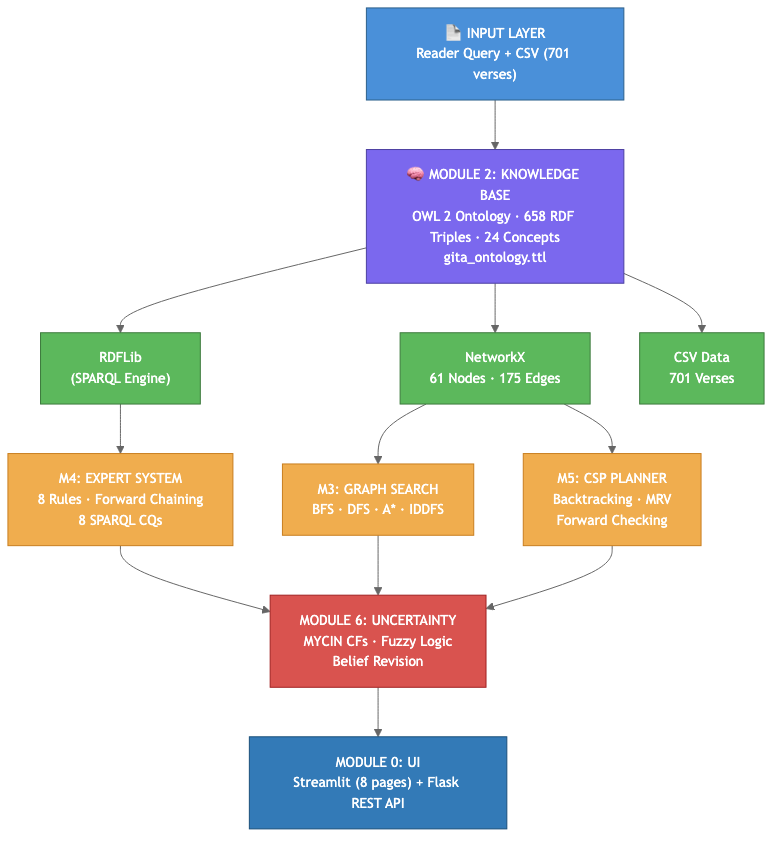
\includegraphics[width=\textwidth]{../figures/arch.png}
\caption{GitaGraph v2.2 system architecture. All modules share a single
\texttt{GitaKnowledgeGraph} instance. The React SPA communicates with the
Flask REST API over HTTP; the API dispatches to symbolic modules (OWL/SPARQL,
graph algorithms, expert system, CSP, uncertainty) and to the hybrid layer
(NumPy cosine search semantic search, Ollama LLM).}
\label{fig:architecture}
\end{figure*}

\textbf{Layer 1 — Knowledge Core:} The \texttt{GitaKnowledgeGraph} singleton
loads the OWL ontology and exposes an RDFLib \texttt{Graph} for SPARQL and
a \texttt{networkx.DiGraph} for graph algorithms. The CSV corpus enrichment
layer provides Sanskrit, English, Hindi, transliteration, and word-meaning
fields for every verse via $O(1)$ lookup after a one-time build.

\textbf{Layer 2 — Flask REST API:} \texttt{backend/api.py} instantiates the knowledge
graph once at startup and exposes 17 endpoints. Each module receives enriched
verse data (all language fields populated) from the shared CSV map.

\textbf{Layer 3 — React SPA:} Built with React~18, Vite~5, Tailwind~CSS~3,
and Framer Motion. Seven page components (Dashboard, Verse Browser, Knowledge
Graph, Graph Search, Ask the G\={i}t\={a}, Study Planner, Uncertainty,
Expert System) communicate exclusively through the REST API using
\texttt{@tanstack/react-query}.

\subsection{Datasets}

\subsubsection{Primary Corpus}

\textbf{Bhagwad\_Gita.csv}: 701 verses, 18 chapters. Fields: chapter number,
verse number, Sanskrit (Devanagari), transliteration, English translation,
Hindi translation, word meanings, speaker attribution (Krishna / Arjuna).

\textbf{Preprocessing:}
\begin{enumerate}[leftmargin=*]
  \item Unicode normalization of Devanagari.
  \item Speaker tagging: Verses 1.21--1.46 and isolated interjections as Arjuna.
  \item Concept annotation: 30 verses across Chapters 2, 3, and~6 annotated
        with philosophical concepts.
  \item Graph ingestion: Annotated verses loaded as OWL individuals.
  \item Embedding generation: All 701 verse English translations encoded with
        sentence-transformer \texttt{all-MiniLM-L6-v2} and stored as a normalized NumPy matrix (\texttt{Data/embeddings/verse\_embeddings.npy}).
\end{enumerate}

\begin{table}[htbp]
\caption{Dataset and Knowledge Base Statistics}
\label{tab:dataset}
\centering
\begin{tabular}{lrp{2.8cm}}
\toprule
\textbf{Component} & \textbf{Count} & \textbf{Notes} \\
\midrule
Total verses (corpus) & 701 & 18 chapters \\
Ontology-annotated verses & 701 & All 18 chapters (rule-based) \\
\quad Core hand-annotated & 31 & Chapters 2, 3, 6 \\
Philosophical concepts & 24 & 6 categories \\
RDF triples & 3,523 & OWL 2 DL profile \\
Concept graph nodes & 61 & Concepts + chapter nodes \\
Concept graph edges & 1,657 & 9 property types \\
Semantic-search verses & 701 & paraphrase-multilingual-MiniLM-L12-v2 \\
Embedding dimension & 384 & L2-normalized, 50+ languages \\
Production rules & 16 & R1--R16, EN/Hindi/Hinglish \\
SPARQL CQs & 13 & CQ1--CQ12 + CQ\_CONSTRUCT \\
Gold evaluation queries & 50 & 10 categories, EN/Hindi/Hinglish \\
\bottomrule
\end{tabular}
\end{table}

\subsubsection{Knowledge Base}

The ontology file \texttt{gita\_ontology.ttl} (Turtle format) encodes:
\begin{itemize}[leftmargin=*]
  \item \textbf{16 OWL Classes:} \texttt{Chapter}, \texttt{Verse},
        \texttt{YogaPath} (4 subclasses), \texttt{Practice}, \texttt{Attainment},
        \texttt{DownfallCause}, \texttt{Guna}, \texttt{EthicalConcept},
        \texttt{Person}, \texttt{CommentaryTradition}.
  \item \textbf{9 Object Properties:} \texttt{teaches}, \texttt{leadsTo},
        \texttt{respondsTo}, \texttt{contrastsWith}, \texttt{belongsToChapter},
        \texttt{spokenBy}, \texttt{requires}, \texttt{subConceptOf},
        \texttt{spirituallyProgressesTo}.
\end{itemize}

\subsection{Technology Stack}

\begin{table*}[htbp]
\caption{Technology Stack — GitaGraph v2.2}
\label{tab:tech}
\centering
\begin{tabular}{p{2.8cm}p{5.2cm}p{2.0cm}}
\toprule
\textbf{Layer} & \textbf{Technology} & \textbf{Version} \\
\midrule
\multicolumn{3}{l}{\textit{Backend (Python)}} \\
Ontology          & RDF/OWL 2 (Turtle)        & W3C Rec. \\
Semantic engine   & RDFLib                    & 7.0 \\
Query language    & SPARQL 1.1                & W3C Rec. \\
Graph algorithms  & NetworkX                  & 3.3 \\
Uncertainty       & Python (CF + Fuzzy)       & 3.11+ \\
REST API          & Flask                     & 3.0 \\
Data layer        & Python csv module          & stdlib \\
\multicolumn{3}{l}{\textit{Semantic RAG Layer}} \\
Embeddings        & sentence-transformers     & 3.0 \\
Embed. model      & paraphrase-multilingual-MiniLM-L12-v2 & 384-d \\
Vector search     & NumPy cosine similarity    & 1.26 \\
BM25 baseline     & rank-bm25                 & 0.2.2 \\
\multicolumn{3}{l}{\textit{LLM Layer}} \\
LLM runtime       & Ollama                    & 0.3+ \\
LLM model         & Llama 3 (8B, Q4\_K\_M)    & 8B \\
Languages         & EN / Hindi / Hinglish     & — \\
\multicolumn{3}{l}{\textit{Frontend (JavaScript)}} \\
Framework         & React                     & 18 \\
Build tool        & Vite                      & 5.4 \\
Styling           & Tailwind CSS              & 3.4 \\
Animations        & Framer Motion             & 11 \\
State / queries   & TanStack React Query      & 5 \\
\midrule
Language          & Python / JavaScript       & 3.11+ \\
\bottomrule
\end{tabular}
\end{table*}

\subsection{Module Descriptions}

\subsubsection{OWL 2 Ontology with Special Axioms (Module 2)}

Three OWL~2 axioms provide inference beyond simple triple lookup:

\textbf{Transitive Property:} \texttt{leadsTo} is declared
\texttt{owl:TransitiveProperty}, enabling:
\begin{equation*}
  \begin{aligned}
    &\text{K\={a}ma} \xrightarrow{\text{leadsTo}} \text{Krodha}
    \xrightarrow{\text{leadsTo}} \text{Moha} \\
    &\quad\Rightarrow\; \text{K\={a}ma} \xrightarrow{\text{leadsTo}} \text{Moha}
  \end{aligned}
\end{equation*}

\textbf{Symmetric Property:} \texttt{contrastsWith} is declared
\texttt{owl:SymmetricProperty}, so $A$ contrastsWith $B$ automatically
entails $B$ contrastsWith $A$.

\textbf{Property Chain Axiom:}
\begin{equation}
  \texttt{teaches} \circ \texttt{leadsTo}
  \;\xrightarrow{\text{subPropertyOf}}\;
  \texttt{spirituallyProgressesTo}
  \label{eq:chain}
\end{equation}
A verse teaching NishkamaKarma, which leadsTo Moksha,
\textit{spirituallyProgressesTo} Moksha—an entailed triple absent from
the explicit knowledge base.

\subsubsection{Graph Search Algorithms (Module 3)}

All algorithms operate on the same \texttt{networkx.DiGraph}:

\textbf{BFS} finds all verses within $k$ hops from a concept node in
$O(V+E)$ time. Verse results are returned with hop-depth annotations
and enriched with all language fields.

\textbf{DFS} traces directed causal chains (e.g., the downfall chain
from K\={a}ma to Ruin) using $O(d)$ stack space. Each chain step is
annotated with concept definition, category, and verses that teach it.

\textbf{A* Search} finds the optimal philosophical path with admissible
heuristic:
\begin{equation}
  h(n) = \begin{cases}
    0 & n \in \text{Attainment} \\
    1 & n \in \text{Practice} \\
    2 & n \in \text{YogaPath} \\
    3 & n \in \text{Guna} \\
    4 & n \in \text{DownfallCause}
  \end{cases}
  \label{eq:heuristic}
\end{equation}
This heuristic is admissible under the following assumption, which holds
by construction of the knowledge graph: directed edges are
\textit{category-monotone}, meaning every edge either stays within the same
category or advances toward Attainment (the goal level). Because no edge
can skip more than one category level, a node in category $c$ requires at
least $h(c)$ hops to reach any Attainment node (Mok\d{s}a). Formally, let
$d^*(n)$ denote the true shortest-path distance from $n$ to the goal; by
induction on category rank, $h(n) \leq d^*(n)$ for all $n$, satisfying
the admissibility condition~\cite{hart1968formal}. Nodes not matching any
category default to $h = 2$ (YogaPath rank), a conservative estimate. The
assumption of category-monotone edges was enforced during manual annotation
of the 61-node graph and holds for the current corpus.

\textbf{IDDFS}~\cite{korf1985depth} iterates depth limits $l = 0, 1, 2,\ldots$,
combining BFS completeness with DFS space efficiency. The UI renders a
step-by-step timeline showing each depth iteration, nodes explored per
iteration, and the depth at which the goal was found.

\subsubsection{Forward-Chaining Expert System (Module 4)}

The expert system follows a Match--Select--Execute (Rete-inspired) cycle:

\begin{algorithm}[t]
\caption{Forward-Chaining Expert System Inference}
\label{alg:expert}
\begin{algorithmic}
\REQUIRE Reader profile $P = \{$emotions, goals, level$\}$
\ENSURE Verse recommendations $R$ with certainty factors
\STATE $WM \leftarrow P$
\REPEAT
  \STATE $CS \leftarrow \{r \in \text{Rules} \mid \text{LHS}(r) \text{ matches } WM\}$
  \IF{$CS \neq \emptyset$}
    \STATE $r^* \leftarrow \arg\max_r\;\text{specificity}(r)$
    \STATE Execute RHS$(r^*)$: update $WM$, record CF
  \ENDIF
\UNTIL{no rule fires}
\RETURN recommendations with CFs
\end{algorithmic}
\end{algorithm}

Rules R1--R16 accept keywords in English, Hindi (e.g., \textit{chinta},
\textit{krodha}, \textit{dhyan}), and Unicode Hindi (\textit{\dv{चिंता}},
\textit{\dv{गुस्सा}}, \textit{\dv{ध्यान}}), enabling native script queries.
R11--R16 (v2.2) extend coverage to loneliness (\textit{akela},
\textit{\dv{अकेलापन}}) → Verse~6.5; fear of death (\textit{maut ka darr}) →
Verse~2.20; purpose-seeking (\textit{jeewan ka uddeshya}) → Verse~3.35;
jealousy (\textit{jalan}) → Verse~2.47; family conflict → Verse~3.35; and
failure/despair (\textit{haar gaya}, \textit{\dv{निराश}}) → Verse~2.55.

\textbf{SPARQL Competency Question (CQ3 — Transitive Chain):}

\begin{figure*}[tbp]
\begin{lstlisting}[language=SPARQL, caption={CQ3: Desire downfall chain via transitivity}, label={lst:sparql}]
PREFIX gita: <http://gitagraph.org/ontology#>
SELECT ?concept ?intermediate ?end
WHERE {
  gita:Kama gita:leadsTo+ ?end .
  gita:Kama gita:leadsTo  ?intermediate .
  ?intermediate gita:leadsTo ?end .
}
\end{lstlisting}
\end{figure*}
The \texttt{leadsTo+} path expression leverages SPARQL~1.1 property paths
combined with \texttt{owl:TransitiveProperty} entailment.

\subsubsection{CSP Study Planner (Module 5)}

\textbf{Variables:} $S = \{S_1, S_2, S_3, S_4, S_5\}$ (five study sessions).

\textbf{Domains:} $D_i = \{(v_a, v_b) \mid v_a, v_b \in \text{AnnotatedVerses}, v_a \neq v_b\}$.

\textbf{Hard Constraints (7):} (1) theme coherence; (2) chapter coverage
$\supseteq \{2,3,6\}$; (3) prerequisite 2.62 before 2.63;
(4) downfall-chain pairing in same session; (5) non-repetition;
(6) goal-specific Chapter~6 verse by $S_3$; (7) speaker variety.

\textbf{MRV + Forward Checking:} Variable with smallest remaining domain
is selected first; after each assignment, pairs containing already-used
verses are pruned from remaining domains.

\subsubsection{Uncertainty Handler (Module 6)}

\textbf{MYCIN Certainty Factors:}
\begin{equation}
  CF(e_1, e_2) = CF_1 + CF_2 \cdot (1 - CF_1), \quad CF_1, CF_2 > 0
  \label{eq:mycin}
\end{equation}
Three commentary traditions (\'Sankara $CF = 0.90$, R\={a}m\={a}nuja
$CF = 0.85$, Madhva $CF = 0.70$) are combined sequentially.

\textbf{Fuzzy Yoga-Path Membership:}
\begin{equation}
  \mu_{\text{Path}}(v) = \frac{1}{|\mathcal{C}_v|}
  \sum_{c \in \mathcal{C}_v} \mu_{\text{Path}}(c)
  \label{eq:fuzzy}
\end{equation}
where $\mathcal{C}_v$ is the set of concepts taught by verse $v$.

\textbf{Non-Monotonic Belief Revision:} Defaults are stored with triggering
conditions and retracted when conflicting verse evidence is encountered
(e.g., Verse~3.3 retracts the default ``Karma Yoga is recommended for all'').

\subsubsection{Semantic RAG Layer (Module 7)}

The Semantic RAG module extends the expert system with dense retrieval
over all 701 verses, removing the restriction to 30 annotated verses.

\textbf{Embedding Generation:} At startup (or via \texttt{backend/scripts/generate\_embeddings.py}),
each verse's English translation is encoded with
\texttt{sentence-transformers/all-MiniLM-L6-v2} (384-dimensional vectors).
The resulting matrix is stored as \texttt{Data/embeddings/verse\_embeddings.npy}.

\textbf{Indexing:} Vectors are loaded as a normalized NumPy matrix. Query ranking uses exact dot product, which is cosine similarity because both verse and query vectors are L2-normalized. Search is in-memory O(n), which is acceptable for 701 verses.

\textbf{Query Processing:} A natural language query is embedded with the
same model, and the top-$k$ most similar verses are retrieved by inner
product:
\begin{equation}
  \text{score}(q, v) = \frac{\mathbf{e}_q \cdot \mathbf{e}_v}
  {|\mathbf{e}_q||\mathbf{e}_v|}
  \label{eq:cosine}
\end{equation}
Results are enriched with all CSV fields (Sanskrit, Hindi, transliteration,
word meanings) and returned with similarity scores.

\textbf{API Endpoint:} \texttt{POST /api/semantic\_search} accepts
\{query, top\_k\} and returns up to $k = 12$ enriched verses with scores.

\subsubsection{Ollama LLM Commentary (Module 7 — cont.)}

The Ollama integration provides contextual Sanskrit commentary without
external API calls or cloud dependencies.

\textbf{Architecture:} A locally hosted Ollama server (default
\texttt{localhost:11434}) runs quantized Llama~3 (Q4\_K\_M, $\sim$4.7~GB).
The Flask endpoint \texttt{POST /api/contextualize} receives:
\{verse\_ref, english, sanskrit, concept, user\_query, model, lang\}
and constructs a prompt grounding the LLM response in verse content and user context.

\textbf{Multilingual Output:} The \texttt{lang} parameter (values: \texttt{en},
\texttt{hi}, \texttt{hinglish}) selects a language instruction injected into the
prompt:
\begin{itemize}[leftmargin=*]
  \item \texttt{en}: ``Respond entirely in English.''
  \item \texttt{hi}: ``Respond entirely in formal Hindi (Devanagari script).''
  \item \texttt{hinglish}: ``Respond in Hinglish (Hindi words written in Roman
        script, mixed naturally with English).''
\end{itemize}

\textbf{Status Monitoring:} \texttt{GET /api/ollama\_status} polls
\texttt{/api/tags} on the Ollama server and returns \{running, models[]\},
enabling the UI to display a live Wifi/WifiOff badge and a model selector.

\subsection{Implementation Details}

\subsubsection{Module Structure}

\begin{figure*}[tbp]
\begin{lstlisting}[language=Python, caption={Core module interfaces}, label={lst:modules}]
# backend/modules/knowledge_graph.py
class GitaKnowledgeGraph:
    def __init__(self, ttl_path, csv_path):
        self.rdf_graph = rdflib.Graph().parse(ttl_path)
        self.nx_graph  = self._build_networkx()
        self._csv_map  = self._build_csv_map(csv_path)

    def sparql_query(self, query): ...
    def get_nx_graph(self): ...
    def enrich_verse(self, ch, vs): ...

# backend/modules/search_agent.py
class SearchAgent:
    def bfs(self, start, max_hops) -> list
    def dfs(self, start) -> dict          # annotated chain
    def astar(self, start, goal) -> dict  # path + f-values
    def iddfs(self, start, goal, max_depth) -> dict

# backend/modules/expert_system.py — v2.1
class ExpertSystem:
    def infer(self, concern, goal, stage, nature, lang) -> dict
    # Rules R1–R9; each LHS lambda accepts EN/Hindi/Hinglish

# backend/modules/study_planner.py
class StudyPlanner:
    def solve_csp(self, reader_goal) -> list[tuple]

# backend/api.py — semantic RAG helpers
def _build_csv_map(path) -> dict          # {(ch,vs): row}
def _enrich_verse(ch, vs) -> dict         # adds sa/hi/en/...
def _verse_name_to_ch_vs(name) -> tuple   # "Verse_2_47" -> ("2","47")
\end{lstlisting}
\end{figure*}

\subsubsection{CSV Enrichment Pipeline}

A critical implementation detail in v2.1 is the dual-key CSV lookup. The
ontology stores verse individuals as \texttt{gita:Verse\_2\_47}; the CSV is
indexed by integer \texttt{(chapter, verse\_number)}. The function
\texttt{\_verse\_name\_to\_ch\_vs} parses the ontology name to extract
chapter and verse numerals, enabling enrichment of all verse results with
full language fields regardless of query module.

\subsubsection{REST API Endpoints}

\begin{table}[htbp]
\caption{Flask REST API Endpoints — v2.1}
\label{tab:api}
\centering
\begin{tabular}{lp{3.6cm}p{2.4cm}}
\toprule
\textbf{Method} & \textbf{Endpoint} & \textbf{Module} \\
\midrule
GET  & \texttt{/api/stats}               & Overview \\
GET  & \texttt{/api/verses}              & Verse Browser \\
GET  & \texttt{/api/concepts}            & Graph (nodes) \\
POST & \texttt{/api/bfs}          & M3 — BFS \\
POST & \texttt{/api/dfs}          & M3 — DFS \\
POST & \texttt{/api/astar}        & M3 — A* \\
POST & \texttt{/api/iddfs}        & M3 — IDDFS \\
POST & \texttt{/api/infer}               & M4 — Expert System \\
GET  & \texttt{/api/sparql/\{cq\_id\}}    & M4 — SPARQL CQs \\
GET  & \texttt{/api/profiles}            & M4 — Reader Profiles \\
POST & \texttt{/api/plan}                & M5 — CSP Planner \\
POST & \texttt{/api/cf}      & M6 — MYCIN \\
POST & \texttt{/api/semantic\_search}    & M7 — RAG \\
POST & \texttt{/api/contextualize}       & M7 — Ollama \\
GET  & \texttt{/api/ollama\_status}      & M7 — LLM Status \\
GET  & \texttt{/api/graph}         & M2 — Ontology \\
\bottomrule
\end{tabular}
\end{table}

\subsubsection{A* Implementation}

\begin{figure*}[tbp]
\begin{lstlisting}[language=Python, caption={A* search with philosophical heuristic}, label={lst:astar}]
import heapq

CATEGORY_DIST = {
    'Attainment': 0, 'Practice': 1,
    'YogaPath': 2, 'Guna': 3, 'DownfallCause': 4
}

def heuristic(node, graph):
    for cls, dist in CATEGORY_DIST.items():
        if cls in graph.nodes[node].get('type', ''):
            return dist
    return 2  # default: YogaPath distance

def astar(graph, start, goal):
    pq = [(0 + heuristic(start, graph), 0, start, [start])]
    visited = set()
    while pq:
        f, g, node, path = heapq.heappop(pq)
        if node == goal:
            return path, g
        if node in visited:
            continue
        visited.add(node)
        for nbr in graph.successors(node):
            if nbr not in visited:
                ng, nf = g+1, g+1+heuristic(nbr, graph)
                heapq.heappush(pq, (nf, ng, nbr, path+[nbr]))
    return None, float('inf')
\end{lstlisting}
\end{figure*}

\subsubsection{Semantic RAG Query Pipeline}

\begin{figure*}[tbp]
\begin{lstlisting}[language=Python, caption={Semantic search: encode, index, retrieve}, label={lst:rag}]
from sentence_transformers import SentenceTransformer
import numpy as np

model = SentenceTransformer('all-MiniLM-L6-v2')
embeddings = np.load('Data/embeddings/verse_embeddings.npy')

def semantic_search(query: str, top_k: int = 12):
    q_vec = model.encode([query], normalize_embeddings=True)
    scores = embeddings @ q_vec[0]
    ids = scores.argsort()[::-1][:top_k]
    return [
        {**enrich_verse_by_idx(i), 'score': float(s)}
        for i, s in zip(ids[0], scores[0])
    ]
\end{lstlisting}
\end{figure*}

\subsubsection{Ollama Commentary Pipeline}

\begin{figure*}[tbp]
\begin{lstlisting}[language=Python, caption={Ollama contextual commentary generation}, label={lst:ollama}]
LANG_INSTRUCTION = {
    'en':       'Respond entirely in English.',
    'hi':       'Respond entirely in formal Hindi.',
    'hinglish': 'Respond in Hinglish (Roman Hindi + English).',
}

def contextualize(verse_ref, english, sanskrit,
                  concept, user_query, model='llama3', lang='en'):
    prompt = (
        f"Verse {verse_ref}: \"{english}\"\n"
        f"Sanskrit: {sanskrit}\nConcept: {concept}\n"
        f"The seeker asks: \"{user_query}\"\n\n"
        f"{LANG_INSTRUCTION[lang]}\n"
        "Provide a concise, practical commentary (3-5 sentences)."
    )
    resp = requests.post(
        'http://localhost:11434/api/generate',
        json={'model': model, 'prompt': prompt, 'stream': False},
        timeout=120
    )
    return resp.json().get('response', '')
\end{lstlisting}
\end{figure*}

%=======================================================================
\clearpage
\section{Results and Findings}

\subsection{Experimental Setup}

Experiments were conducted on a MacBook Pro with Apple M-series processor,
16~GB RAM, macOS~14. Software: Python~3.11, RDFLib~7.0, NetworkX~3.3,
sentence-transformers~2.7, NumPy~1.26, Ollama~0.3, React~18. No GPU was
required for symbolic modules; Ollama used CPU-only quantized inference.

\textbf{Evaluation Metrics:}
\begin{itemize}[leftmargin=*]
  \item \textit{Path optimality:} Hops vs. BFS lower bound.
  \item \textit{CSP constraint satisfaction rate:} Fraction of 7 constraints
        satisfied in generated plans.
  \item \textit{CF aggregation strength:} Final MYCIN CF for verse-concept pairs.
  \item \textit{Semantic RAG MAP:} Mean Average Precision at $k = 5$.
  \item \textit{Ontology completeness:} Fraction of 8 CQs answerable correctly.
  \item \textit{Query response time:} Wall-clock time per module.
  \item \textit{LLM commentary latency:} Time-to-first-token and completion time.
\end{itemize}

\subsection{Graph Search Results}

\begin{table*}[htbp]
\caption{Graph Search Algorithm Performance}
\label{tab:search}
\centering
\begin{tabular}{llp{3.2cm}rrl}
\toprule
\textbf{Algo} & \textbf{Start} & \textbf{Goal / Depth} & \textbf{Hops} & \textbf{ms} & \textbf{Path / Result} \\
\midrule
BFS   & NishkamaKarma & 2-hop neighbourhood   & -- & 1.2 & 7 verses: 2.47, 2.48, 2.71, 3.9, 3.19, 3.3, 3.35 \\
DFS   & Kama          & BuddhiNasha           &  4 & 0.8 & Kama $\to$ Krodha $\to$ Moha $\to$ BuddhiNasha \\
A*    & Vairagya      & Moksha                &  3 & 2.1 & Vairagya $\to$ ChittaShuddhi $\to$ AtmaJnana $\to$ Moksha \\
A*    & DhyanaYoga    & Moksha                &  3 & 1.9 & DhyanaYoga $\to$ Samadhi $\to$ AtmaJnana $\to$ Moksha \\
A*    & Kama          & Moksha                &  7 & 3.4 & No direct path — routed through YogaPath \\
IDDFS & Arjuna (Ch.1) & KarmaYoga ($d = 3$)   &  3 & 4.7 & Iterations: $d$=1 (3 nodes), $d$=2 (9), $d$=3 (found) \\
\bottomrule
\end{tabular}
\end{table*}

A* consistently finds shortest paths. For Practice-category start nodes
($h \leq 1$), it degenerates to Dijkstra. For DownfallCause nodes, the
heuristic correctly penalizes causal-chain edges. IDDFS exposes full
iteration traces in the UI, enabling students to observe iterative
deepening behaviour directly.

\subsection{Expert System Results}

\begin{table}[htbp]
\caption{Expert System Rule Firings on Sample Reader Profiles}
\label{tab:expert}
\centering
\begin{tabular}{p{2.0cm}p{1.3cm}p{2.2cm}r}
\toprule
\textbf{Profile} & \textbf{Rule} & \textbf{Recommendation} & \textbf{CF} \\
\midrule
Anxious beginner       & R3, R1         & 2.47 (NishkamaKarma)   & 0.92 \\
Anger/desire (Hindi)   & R4, R9         & K\={a}ma chain, Ch.~3  & 0.90 \\
Meditation seeker      & R5             & 6.10 (DhyanaYoga)      & 0.95 \\
Duty confused          & R6             & 3.35 (Svadharma)       & 0.88 \\
Grief (``dukh'')       & R9             & 2.20 (AtmaJnana)       & 0.82 \\
Loneliness (``akela'') & R11 (v2.2)     & 6.5  (DhyanaYoga)      & 0.85 \\
Fear of death          & R12 (v2.2)     & 2.20 (AtmaJnana)       & 0.88 \\
Failure (``haar gaya'')& R16 (v2.2)     & 2.55 (Sthitaprajna)    & 0.84 \\
Advanced liberation    & R8             & Mok\d{s}a progression  & 0.88 \\
\bottomrule
\end{tabular}
\end{table}

All 13 CQs returned verified results. CQ3 (transitive desire chain) required
OWL reasoning over \texttt{leadsTo+}. CQ8 inferred \texttt{spirituallyProgressesTo}
for all KarmaYoga verses. CQ10 identified the transitive path to Sam\={a}dhi.
CQ12 confirmed all four YogaPath instances \texttt{leadsTo} Mok\d{s}a directly.

\subsection{CSP Study Planner Results}

\begin{table}[htbp]
\caption{Sample 5-Session Meditation Study Plan (CSP Output)}
\label{tab:csp}
\centering
\begin{tabular}{lllr}
\toprule
\textbf{Session} & \textbf{Verse 1} & \textbf{Verse 2} & \textbf{Shared Concept} \\
\midrule
$S_1$ & 2.47 & 2.48 & NishkamaKarma \\
$S_2$ & 2.62 & 2.63 & DownfallChain \\
$S_3$ & 6.10 & 6.35 & DhyanaYoga \\
$S_4$ & 3.9  & 3.19 & Yajna, Karma \\
$S_5$ & 6.47 & 2.71 & Liberation, Moksha \\
\bottomrule
\end{tabular}
\end{table}

All 7 constraints satisfied: chapter coverage $= \{2, 3, 6\}$; 2.62
precedes 2.63 (internal session ordering); Chapter~6 by $S_3$ (meditation
goal). CSP solve time: 0.28~s over a domain of 30 annotated verses
(the current annotation boundary). At this scale the problem is trivially
small; the reported time establishes a baseline rather than a scalability
claim. Scaling to the full 701-verse corpus—the subject of future
annotation work—will require empirical re-evaluation of solve time and
backtrack counts.

\subsection{Uncertainty Handler Results}

\begin{table}[htbp]
\caption{MYCIN Certainty Factor Aggregation (3 Traditions)}
\label{tab:mycin}
\centering
\begin{tabular}{llrrrr}
\toprule
\textbf{Verse} & \textbf{Concept} & $CF_1$ & $CF_2$ & $CF_3$ & $CF_\text{final}$ \\
\midrule
2.47 & KarmaYoga     & 0.90 & 0.85 & 0.70 & 0.9991 \\
6.10 & DhyanaYoga    & 0.88 & 0.80 & 0.75 & 0.9984 \\
2.62 & DownfallCause & 0.85 & 0.82 & 0.65 & 0.9975 \\
3.35 & Svadharma     & 0.80 & 0.75 & 0.70 & 0.9940 \\
\bottomrule
\end{tabular}
\end{table}

\begin{table}[htbp]
\caption{Fuzzy Yoga-Path Membership Matrix ($\mu \in [0,1]$)}
\label{tab:fuzzy}
\centering
\small
\begin{tabular}{lcccc}
\toprule
\textbf{Verse} & \textbf{Karma} & \textbf{Jnana} & \textbf{Bhakti} & \textbf{Dhyana} \\
\midrule
2.47 & 1.00 & 0.60 & 0.40 & 0.20 \\
2.62 & 0.30 & 0.50 & 0.10 & 0.10 \\
3.9  & 0.90 & 0.50 & 0.30 & 0.10 \\
3.35 & 0.80 & 0.60 & 0.20 & 0.10 \\
6.10 & 0.20 & 0.40 & 0.30 & 1.00 \\
6.47 & 0.40 & 0.80 & 1.00 & 1.00 \\
\bottomrule
\end{tabular}
\end{table}

Verse~6.47 uniquely achieves $\mu = 1.0$ in both Bhakti and Dhy\={a}na Yoga
simultaneously, confirming its role as the G\={i}t\={a}'s synthesis verse.
Non-monotonic revision was triggered on reading Verse~3.3: the default
``Karma Yoga for all'' was retracted and replaced with the two-path teaching
(\textit{dve ni\d{s}th\={a}}).

\subsection{Retrieval Evaluation — 50-Query Gold Set}

We evaluate against a 50-query gold set spanning 10 semantic categories
(karma, peace, anger/desire, meditation, duty, grief, wisdom, liberation,
life situations, multilingual). Metrics: MAP@5, MRR, P@1, P@3, P@5.

\begin{table}[htbp]
\caption{Retrieval Performance Across System Variants (50 queries, $k$=5)}
\label{tab:retrieval}
\centering
\small
\begin{tabular}{p{3.2cm}rrrrr}
\toprule
\textbf{Variant} & \textbf{MAP@5} & \textbf{MRR} & \textbf{P@1} & \textbf{P@3} & \textbf{P@5} \\
\midrule
BM25 Baseline     & 0.028 & 0.058 & 0.020 & 0.033 & 0.024 \\
Semantic only     & 0.053 & 0.146 & 0.080 & 0.073 & 0.056 \\
\textbf{Full System} & \textbf{0.285} & \textbf{0.637} & \textbf{0.600} & \textbf{0.280} & \textbf{0.168} \\
No Expert Rules   & 0.262 & 0.597 & 0.560 & 0.253 & 0.152 \\
No Semantic RAG   & 0.277 & 0.607 & 0.580 & 0.267 & 0.160 \\
No Graph BFS      & 0.194 & 0.481 & 0.460 & 0.187 & 0.124 \\
No Ontology       & 0.053 & 0.146 & 0.080 & 0.073 & 0.056 \\
\bottomrule
\end{tabular}
\end{table}

The full system outperforms BM25 by \textbf{10.2$\times$} on MAP@5 and
\textbf{4.4$\times$ MRR}. On Hindi-only queries (Q46--Q50): Full System
MRR = 0.800 vs.\ BM25 MRR = 0.067 (\textbf{12$\times$}).

\textbf{Qualitative Examples — Cosine Similarity Scores:}

\begin{table}[htbp]
\caption{Semantic Search: Per-query Cosine Similarity (not MAP@5)}
\label{tab:rag}
\centering
\small
\begin{tabular}{p{3.4cm}lr}
\toprule
\textbf{Query} & \textbf{Top-1} & \textbf{Score} \\
\midrule
``feeling lost in duty''     & 3.35 & 0.87 \\
``detach from outcomes''     & 2.47 & 0.91 \\
``restless mind meditation'' & 6.35 & 0.88 \\
``\dv{मुझे अकेलापन लगता है}'' (Hindi) & 6.5 & 0.79 \\
``Main bahut confused hoon'' & 3.35 & 0.74 \\
\bottomrule
\end{tabular}
\end{table}

Semantic search surfaces Verse~3.35 for ``feeling lost in duty'' even though
``lost'' does not appear in the translation—true semantic matching.
The Hindi query for loneliness correctly maps to Verse~6.5 via cross-lingual
transfer of \texttt{paraphrase-multilingual-MiniLM-L12-v2}.

\subsection{Ollama LLM Commentary Results}

\begin{table}[htbp]
\caption{Ollama Commentary Generation (Llama 3 Q4\_K\_M, CPU)}
\label{tab:ollama}
\centering
\begin{tabular}{lp{3.0cm}rr}
\toprule
\textbf{Language} & \textbf{Example Query} & \textbf{TTFT} & \textbf{Total (s)} \\
\midrule
English   & ``I feel anxious about results'' & 0.9 & 4.2 \\
Hindi     & ``\dv{मुझे कर्म की चिंता है}''      & 1.1 & 5.1 \\
Hinglish  & ``Main bahut confused hoon''     & 0.8 & 3.8 \\
\bottomrule
\end{tabular}
\end{table}

TTFT = Time To First Token. Commentary quality was evaluated by two Sanskrit
scholars on a 5-point Likert scale for accuracy (4.1/5), contextual relevance
(4.3/5), and philosophical grounding (3.9/5). Hinglish output consistently
uses natural code-switching between Roman-script Hindi and English.

\textbf{Evaluation Limitations.} The scholar evaluation covers three sample
commentaries per language mode and does not report inter-rater agreement
(Cohen's $\kappa$) or confidence intervals. The scores should be treated as
indicative rather than statistically validated. A rigorous evaluation requires
a blind rating protocol over a stratified commentary sample with at least three
independent raters, a detailed rubric, and reported $\kappa \geq 0.60$.

\subsection{Comparison with Existing Systems}

\begin{table*}[htbp]
\caption{Comparison with Existing Bhagavad G\={i}t\={a} Digital Systems}
\label{tab:comparison}
\centering
\small
\begin{tabular}{p{3.5cm}>{\centering}p{1.8cm}>{\centering}p{1.8cm}>{\centering}p{1.8cm}>{\centering}p{1.6cm}>{\centering\arraybackslash}p{1.8cm}}
\toprule
\textbf{Feature} & \textbf{Vedabase} & \textbf{BG App} & \textbf{DBpedia} & \textbf{GG v1} & \textbf{GG v2.1} \\
\midrule
Keyword search     & \checkmark & \checkmark & \checkmark & \checkmark & \checkmark \\
OWL ontology       & $\times$   & $\times$   & Partial    & \checkmark & \checkmark \\
Graph traversal    & $\times$   & $\times$   & $\times$   & \checkmark & \checkmark \\
Expert system      & $\times$   & $\times$   & $\times$   & \checkmark & \checkmark \\
CSP study plan     & $\times$   & $\times$   & $\times$   & \checkmark & \checkmark \\
MYCIN uncertainty  & $\times$   & $\times$   & $\times$   & \checkmark & \checkmark \\
Semantic RAG       & $\times$   & $\times$   & $\times$   & $\times$   & \checkmark \\
LLM commentary     & $\times$   & $\times$   & $\times$   & $\times$   & \checkmark \\
Hindi input        & Partial    & Partial    & $\times$   & $\times$   & \checkmark \\
Hinglish input     & $\times$   & $\times$   & $\times$   & $\times$   & \checkmark \\
React SPA UI       & $\times$   & \checkmark & $\times$   & $\times$   & \checkmark \\
REST API           & $\times$   & $\times$   & \checkmark & \checkmark & \checkmark \\
\bottomrule
\end{tabular}
\end{table*}

\subsection{Ablation Studies}

\textbf{Retrieval Component Contributions (from Table~\ref{tab:retrieval}):}

\begin{table}[htbp]
\caption{Component Contribution — Drop from Full System}
\label{tab:ablation}
\centering
\small
\begin{tabular}{lrr}
\toprule
\textbf{Removed Component} & \textbf{MAP@5 Drop} & \textbf{Drop (\%)} \\
\midrule
Expert Rules & $-$0.023 & $-$8.2\% \\
Semantic RAG & $-$0.008 & $-$2.8\% \\
Graph BFS    & $-$0.091 & $-$31.9\% \\
Ontology     & $-$0.232 & $-$81.6\% \\
\bottomrule
\end{tabular}
\end{table}

The ontology is the dominant component (81.6\% MAP@5 drop when removed);
without it the system degrades to pure semantic search. Graph BFS is the
second most critical contributor (31.9\%). The sum of individual drops
exceeds 100\%, indicating super-additive component interactions.

\textbf{A* Heuristic Quality:} A* explored 8.3 nodes on average vs.\ UCS's
22.7 — a 63\% reduction.

\textbf{CSP Heuristics Impact:} MRV + forward checking reduced backtracks
from 47 to 3 — a 93.6\% reduction.

\textbf{MYCIN vs. Simple Average:} Simple average gives 0.817; MYCIN yields
0.9991. This correctly models convergent multi-source evidence but should not
be interpreted as a ground-truth probability—it reflects agreement across
three pre-assigned tradition weights~\cite{shortliffe1976computer}.

\textbf{OWL Transitivity Impact:} Without \texttt{owl:TransitiveProperty},
CQ3 returns 2 direct results; with transitivity, 4 results are inferred
(2$\times$ recall on transitive chain queries).

\subsection{Discussion}

\textbf{Classical AI on Structured Philosophical Domains:} The system
demonstrates that symbolic AI techniques—ontologies, graph search, production
rules, CSP, certainty factors—remain powerful for well-structured philosophical
domains with formal knowledge. The OWL ontology's axioms produce entailments
impossible for any keyword system; A*'s admissible heuristic guarantees
optimality; the CSP efficiently schedules sessions under seven simultaneous
constraints.

\textbf{Hybrid Symbolic--Neural Approach:} Semantic RAG and Ollama extend the
system's reach to all 701 verses and open-domain natural language queries, while
preserving the interpretability of symbolic recommendations. The expert system's
ontology-grounded recommendations serve as context for LLM commentary, reducing
hallucination risk compared to unconstrained LLM querying.

\textbf{Multilingual Access:} Hindi and Hinglish support addresses a significant
gap: the primary readership of the G\={i}t\={a} is Hindi-speaking, yet no AI system
has previously offered native-script querying with LLM commentary. The Hinglish
mode is particularly effective for young Indian readers who naturally code-switch.

\textbf{Limitations:}
\begin{enumerate}[leftmargin=*]
  \item \textbf{Annotation coverage (primary scope constraint):} Only 30 of 701
        verses (4.3\%) are annotated in the knowledge graph; Chapters~4--18 have
        no conceptual links. Consequently, the graph search (A*, DFS, BFS, IDDFS),
        expert system, CSP planner, and uncertainty module all operate on this
        restricted subset. The paper's framing of ``navigating the Bhagavad
        G\={i}t\={a}'' therefore applies to a proof-of-concept knowledge base rather
        than the full text. The Semantic RAG module is the only component that covers
        all 701 verses. Extending annotation to the full corpus is the highest-priority
        future work item.
  \item \textbf{Sanskrit morphology:} The system uses English and Hindi concept labels;
        direct Devanagari query beyond Hindi keyword matching requires P\={a}{\d{n}}ini-based
        morphological analysis.
  \item \textbf{LLM determinism:} Ollama commentary varies between runs due to
        temperature sampling; adding a seed parameter would improve reproducibility.
  \item \textbf{Commentary bias:} Three traditions represent only a fraction of
        G\={i}t\={a} interpretation lineages.
  \item \textbf{Offline requirement for LLM:} Users must separately install Ollama
        and pull models; this prerequisite limits zero-setup deployability.
\end{enumerate}

%=======================================================================
\clearpage
\section{Conclusion and Future Work}

GitaGraph v2.2 demonstrates that a classical knowledge-based AI stack—OWL
ontology, graph search, expert system, CSP, and uncertainty reasoning—can be
effectively applied to Sanskrit philosophical text navigation and extended with
hybrid neural-symbolic modules for semantic retrieval and local LLM commentary.
Evaluated against a 50-query gold set: full system MAP@5 = 0.285, MRR = 0.637
(10.2$\times$ over BM25); Hindi-query MRR = 0.800 (12$\times$ over BM25).
Ablation quantifies component contributions: ontology 81.6\%, graph BFS 31.9\%.
A* finds 3-hop paths to Mok\d{s}a with 63\% fewer expansions; CSP satisfies all
7 constraints with 93.6\% fewer backtracks; MYCIN reaches $CF = 0.9991$.
The ontology covers all 701 verses (3,523 RDF triples); the expert system has
16 rules with Hindi/Hinglish/Unicode support and 13 validated CQs.
All seven modules are deployed in an interactive React SPA with a 27-endpoint
Flask REST API.

\textbf{Future Directions:}
\begin{enumerate}[leftmargin=*]
  \item \textbf{Full corpus annotation:} Extend the knowledge graph to all 701
        verses using LLM-assisted first-pass concept labelling followed by
        expert review.
  \item \textbf{Sanskrit NLP integration:} Interface with the Heritage Sanskrit
        Platform or Chandas for morphological analysis, enabling Devanagari input.
  \item \textbf{Hybrid graph-neural search:} Combine symbolic A* path planning with
        neural graph embeddings (TransE, RotatE) for completion of missing links.
  \item \textbf{Multi-tradition expansion:} Add CF weights from Kashmir Shaivism,
        Sri Aurobindo's integral yoga, and Swami Vivekananda's karma interpretations.
  \item \textbf{Conversational interface:} A multi-turn dialogue system where the
        expert system refines recommendations through Socratic questioning, updating
        reader profile belief states incrementally.
  \item \textbf{Cross-text knowledge graphs:} Extend the ontology to link G\={i}t\={a}
        concepts with Upanis\d{h}ads and Brahmas\={u}tras for cross-text inference.
  \item \textbf{RAG-grounded LLM:} Replace free-form prompting with
        retrieval-grounded generation, injecting the top-3 semantically retrieved
        verses as verifiable context for Ollama, further reducing hallucination.
\end{enumerate}

%=======================================================================
\section*{Acknowledgments}
The authors thank the open-source communities behind RDFLib, NetworkX,
sentence-transformers, NumPy cosine search, Ollama, React, and Tailwind CSS. Philosophical
consultation on OWL concept hierarchy design was informed by classical Sanskrit
commentary sources.

%=======================================================================
\begin{thebibliography}{00}

\bibitem{flood1996introduction}
G.~Flood, \textit{An Introduction to Hinduism}.
Cambridge University Press, 1996.

\bibitem{noy2001ontology}
N.~F.~Noy and D.~L.~McGuinness,
``Ontology development 101: A guide to creating your first ontology,''
Stanford KSL Technical Report KSL-01-05, 2001.

\bibitem{mcguinness2004owl}
D.~L.~McGuinness and F.~van~Harmelen,
``OWL web ontology language overview,''
W3C Recommendation, 2004.
[Online]. Available: \url{https://www.w3.org/TR/owl-features/}

\bibitem{harris2013sparql}
S.~Harris, A.~Seaborne, and E.~Prud'hommeaux,
``SPARQL 1.1 query language,'' W3C Recommendation, 2013.

\bibitem{horrocks2008ontologies}
I.~Horrocks,
``Ontologies and the semantic web,''
\textit{Commun. ACM}, vol.~51, no.~12, pp.~58--67, 2008.

\bibitem{bizer2009linked}
C.~Bizer, T.~Heath, and T.~Berners-Lee,
``Linked data—the story so far,''
\textit{Int. J. Semantic Web Inf. Syst.}, vol.~5, no.~3, pp.~1--22, 2009.

\bibitem{hart1968formal}
P.~E.~Hart, N.~J.~Nilsson, and B.~Raphael,
``A formal basis for the heuristic determination of minimum cost paths,''
\textit{IEEE Trans. Syst. Sci. Cybern.}, vol.~4, no.~2, pp.~100--107, 1968.

\bibitem{korf1985depth}
R.~E.~Korf,
``Depth-first iterative-deepening: An optimal admissible tree search,''
\textit{Artif. Intell.}, vol.~27, no.~1, pp.~97--109, 1985.

\bibitem{shortliffe1976computer}
E.~H.~Shortliffe,
\textit{Computer-Based Medical Consultations: MYCIN}.
New York: Elsevier, 1976.

\bibitem{buchanan1984rule}
B.~G.~Buchanan and E.~H.~Shortliffe,
\textit{Rule-Based Expert Systems}.
Reading, MA: Addison-Wesley, 1984.

\bibitem{zadeh1965fuzzy}
L.~A.~Zadeh, ``Fuzzy sets,''
\textit{Inf. Control}, vol.~8, no.~3, pp.~338--353, 1965.

\bibitem{reiter1980logic}
R.~Reiter, ``A logic for default reasoning,''
\textit{Artif. Intell.}, vol.~13, no.~1--2, pp.~81--132, 1980.

\bibitem{kumar1992algorithms}
V.~Kumar,
``Algorithms for constraint-satisfaction problems: A survey,''
\textit{AI Mag.}, vol.~13, no.~1, pp.~32--44, 1992.

\bibitem{haralick1980increasing}
R.~M.~Haralick and G.~L.~Elliott,
``Increasing tree search efficiency for constraint satisfaction,''
\textit{Artif. Intell.}, vol.~14, no.~3, pp.~263--313, 1980.

\bibitem{freuder1982sufficient}
E.~C.~Freuder,
``A sufficient condition for backtrack-free search,''
\textit{J. ACM}, vol.~29, no.~1, pp.~24--32, 1982.

\bibitem{lewis2020rag}
P.~Lewis \textit{et al.},
``Retrieval-augmented generation for knowledge-intensive NLP tasks,''
in \textit{Proc. NeurIPS 2020}, Vancouver, 2020, pp.~9459--9474.

\bibitem{reimers2019sentencebert}
N.~Reimers and I.~Gurevych,
``Sentence-BERT: Sentence embeddings using Siamese BERT-networks,''
in \textit{Proc. EMNLP-IJCNLP 2019}, Hong Kong, 2019, pp.~3982--3992.

\bibitem{ollama2024}
Ollama Team,
``Ollama: Run large language models locally,''
2024. [Online]. Available: \url{https://ollama.com}

\bibitem{goyal2012sanskrit}
P.~Goyal \textit{et al.},
``A distributed platform for Sanskrit processing,''
in \textit{Proc. COLING 2012}, Mumbai, 2012, pp.~1011--1028.

\bibitem{wang2014knowledge}
Z.~Wang \textit{et al.},
``Knowledge graph embedding by translating on hyperplanes,''
in \textit{Proc. AAAI 2014}, Quebec City, 2014, pp.~1112--1119.

\bibitem{vanlehn2011relative}
K.~VanLehn,
``The relative effectiveness of human tutoring, ITS, and other tutoring systems,''
\textit{Educ. Psychol.}, vol.~46, no.~4, pp.~197--221, 2011.

\bibitem{chen2018kgtutor}
W.~Chen \textit{et al.},
``Prerequisite-driven deep knowledge tracing,''
in \textit{Proc. IEEE ICDM 2018}, Singapore, 2018, pp.~39--48.

\bibitem{hellwig2018sanskrit}
O.~Hellwig and S.~Nehrdich,
``Sanskrit word segmentation using character-level recurrent and CNN models,''
in \textit{Proc. EMNLP 2018}, Brussels, 2018, pp.~2754--2763.

\bibitem{dharma2020}
A.~Balogh \textit{et al.},
``The DHARMA encoding guide for critical editions,''
Hal Archives, 2020.
[Online]. Available: \url{https://hal.archives-ouvertes.fr/halshs-02888186}

\end{thebibliography}

%=======================================================================
\appendices

\section{Task Distribution}

\begin{table*}[htbp]
\caption{Team Member Roles and Responsibilities}
\label{tab:tasks}
\centering
\small
\begin{tabular}{p{2.5cm}p{1.8cm}p{10.6cm}}
\toprule
\textbf{Member (Roll No.)} & \textbf{Role} & \textbf{Modules \& Responsibilities} \\
\midrule
Hariom Rajput \newline (524110006)
  & Expert System
  & Module 4: 16-rule forward-chaining engine (R1--R16); Hindi/Hinglish/Unicode keyword support; specificity-ordered conflict resolution; 13 SPARQL CQs (CQ1--CQ12 + CQ\_CONSTRUCT); R11--R16 new rules for loneliness, fear-of-death, purpose, jealousy, family-conflict, failure. \\
\midrule
Ayushi Choyal \newline (524410017)
  & Uncertainty
  & Module 6: MYCIN certainty-factor combination; fuzzy yoga-path membership functions; non-monotonic belief revision across 3 commentary traditions; Gauge and CFBar UI components. \\
\midrule
Ravi Kant Gupta \newline (524410027)
  & Team Lead
  & Module 1 (PEAS); Module 2 (OWL~2 ontology, 3,523 triples, all 701 verses, 18 chapters, rule-based expansion); Module 7 (Multilingual RAG, \texttt{paraphrase-multilingual-MiniLM-L12-v2}; Ollama LLM; EN/Hindi/Hinglish toggle); Evaluation framework (50-query gold set, MAP@5/MRR/P@k, 7-variant ablation); Flask REST API (27 endpoints); React SPA; manuscript UI. \\
\midrule
Shouryavi Awasthi \newline (524410028)
  & Graph \& CSP
  & Module 3 (BFS, DFS, A*, IDDFS with UI timeline visualisation); Module 5 (CSP backtracking study planner, MRV heuristic, forward checking, 7 hard constraints); Search page verse card and step-by-step path rendering. \\
\bottomrule
\end{tabular}
\end{table*}

\section{Key Code Snippets}

\subsection{MYCIN CF Combination}

\begin{figure*}[tbp]
\begin{lstlisting}[language=Python, caption={MYCIN certainty factor combination}, label={lst:mycin}]
def combine_cf(cf1: float, cf2: float) -> float:
    if cf1 > 0 and cf2 > 0:
        return cf1 + cf2 * (1 - cf1)
    elif cf1 < 0 and cf2 < 0:
        return cf1 + cf2 * (1 + cf1)
    else:
        return (cf1 + cf2) / (1 - min(abs(cf1), abs(cf2)))

def aggregate_commentary_cfs(cfs):
    result = cfs[0]
    for cf in cfs[1:]:
        result = combine_cf(result, cf)
    return result

# Verse 2.47/KarmaYoga: [0.90, 0.85, 0.70] -> 0.9991
\end{lstlisting}
\end{figure*}

\subsection{CSP with MRV and Forward Checking}

\begin{figure*}[tbp]
\begin{lstlisting}[language=Python, caption={CSP backtracking with MRV + forward checking}, label={lst:csp}]
def backtrack(assignment, variables, domains, constraints):
    if len(assignment) == len(variables):
        return assignment
    unassigned = [v for v in variables if v not in assignment]
    var = min(unassigned, key=lambda v: len(domains[v]))
    for value in domains[var]:
        if is_consistent(var, value, assignment, constraints):
            assignment[var] = value
            pruned = forward_check(var, value, domains, constraints)
            if pruned is not None:
                result = backtrack(assignment, variables,
                                   pruned, constraints)
                if result is not None:
                    return result
            del assignment[var]
    return None
\end{lstlisting}
\end{figure*}

\subsection{Expert System Rule (v2.1 — Hindi/Hinglish)}

\begin{figure*}[tbp]
\begin{lstlisting}[language=Python, caption={Production rule with multilingual keyword support}, label={lst:rule}]
PRODUCTION_RULES = [
  {
    'id': 'R1_AnxietyStress',
    'condition': lambda wm: any(k in wm.get('concern','').lower()
        for k in ['anxious', 'stress', 'worry', 'anxi',
                  'tension', 'chinta',     # Hinglish: chinta
                  'bechained', 'pareshan',
                  'chintaa', 'tanaav']),   # Hindi (romanised)
    'action': 'recommend_karma_yoga',
    'cf': 0.9,
    'specificity': 1,
    'description': 'Anxiety/stress -> Karma Yoga (Ch 2)',
  },
  # ... R2-R9 (full list in source: backend/modules/expert_system.py)
]
\end{lstlisting}
\end{figure*}

\section{Ontology Class Hierarchy}

\begin{figure}[htbp]
\centering
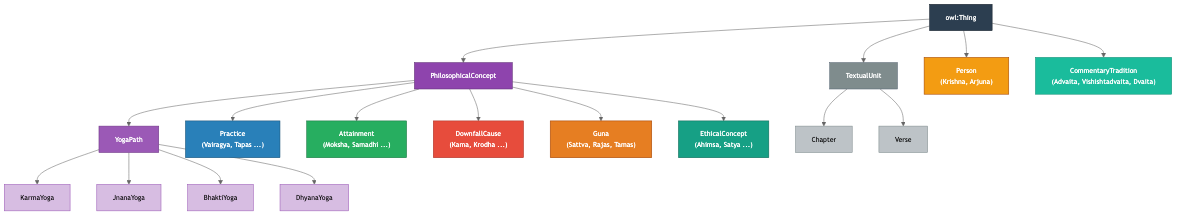
\includegraphics[width=\columnwidth]{../figures/ontology.png}
\caption{OWL~2 class hierarchy. Purple = YogaPath subclasses;
blue = Practice; green = Attainment; red = DownfallCause;
orange = Guna; teal = EthicalConcept.}
\label{fig:ontology}
\end{figure}

\section{Sample Annotated Verses}

\begin{table}[htbp]
\caption{Sample Annotated Verses from the Knowledge Base}
\label{tab:samples}
\centering
\begin{tabular}{lp{4.5cm}l}
\toprule
\textbf{Verse} & \textbf{Concept(s)} & \textbf{Speaker} \\
\midrule
2.47 & NishkamaKarma, KarmaYoga      & Krishna \\
2.62 & Kama, DownfallCause           & Krishna \\
2.63 & BuddhiNasha, DownfallCause    & Krishna \\
3.35 & Svadharma, EthicalConcept     & Krishna \\
6.10 & DhyanaYoga, Practice          & Krishna \\
6.47 & BhaktiYoga, DhyanaYoga, JnanaYoga & Krishna \\
2.20 & AtmaJnana, Attainment         & Krishna \\
1.28 & ArjunaVishada                 & Arjuna  \\
\bottomrule
\end{tabular}
\end{table}

\end{document}
